\chapter{Research outlook}
\label{chap9}

\minitoc

\section{Dynamics of shallow magmatic intrusions}
\label{sec:dynam-shall-magm}

Intermediate-scaled  shallow  magmatic  intrusions  are  the  building
blocks    of    larger    plutons     intruded    into    the    crust
\citep{Petford:2000cc,Glazner:2004gv}. The  first goal of  this thesis
was to explore two important  mechanisms related to magmatic intrusion
emplacement: the effect a temperature-dependent rheology for the magma
and  the  effect of  an  overburden  characterized by  a  non-constant
thickness.   Our approach,  closely combining  theoretical models  and
observations, have  shown successful in reproducing  the leading order
deformation of terrestrial laccoliths and crater-centered intrusions.

\subsection{Toward an understanding of the small-scale dynamics in the
  tip}
\label{sec:perspectives}

In Chapter  \ref{chap2}, \ref{C3-JFM} and \ref{Heating},  we show that
the local condition at the tip of the current controls the dynamics in
the  bending  regime.  For  a  sake  of  simplicity,  we used  a  thin
prewetting film  at the tip to  avoid the requirement of  any boundary
condition at a genuine front. This approach allowed us to get insights
into  the  coupling  between  the   thermal  structure  and  the  flow
itself. In particular, it captures the leading order behavior of these
shallow intrusions.   Nevertheless, a more precise  description of the
mechanisms  operating  at the  scale  of  the  tip might  help  better
characterize the dynamics of both sills and laccoliths.

\subsubsection*{Fluid driven fracture}
\label{sec:caref-descr-tip}

A first step  would be to describe  the tip in term of  a fluid driven
fracture  instead of  the thin  prewetting  film. As  seen in  Section
\ref{C2-Toughness},  linear elastic  fracture mechanics  requires that
the  mode $I$  intensity  factor  $K_I$ equal  a  critical value,  the
fracture toughness  of the wall  rock $K_{c}$, for the  propagation to
occur.  This condition  is usually expressed in term  of an asymptotic
condition      on      the       crack      opening      at      $r=R$
\citep{Savitski:2002gy,Bunger:2005em,Bunger:2007vs,Detournay:2014fk}.

In  such  problem, the  lubrication  equation  is  thus coupled  to  a
description  of  the fracture  opening  based  on the  linear  elastic
fracture mechanics.  \citet{Bunger:2011cb} use  this approach to solve
the problem of  shallow magmatic intrusions and  found similar results
than  \citet{Michaut:2011kg}.  Interestingly,  they needed  values for
the fracture toughness $K_c$ two  or three orders of magnitudes larger
than  laboratory measurements  to agree  with the  observations, which
they attribute to  potentially crack blunting mechanism at  the tip of
laccoliths.  This  observation is consistent with  the rapid formation
of  a  highly viscous  plug  at  the  tip  of the  magmatic  intrusion
described in Chapter \ref{C3-JFM} and \ref{Heating}.

Nevertheless, this model also falls short to reproduce the geometry of
large  mafic sills.   In addition,  more realistic  model should  also
consider the process zone, i.e. the region of plastic rock deformation
near the leading edge of the fracture \citep{Bunger:2008cl}.

\subsubsection*{Gas filled region}
\label{sec:caref-descr-tip}

Furthermore, the large  negative pressure that developed  at the front
might  cause desolved  gasses to  exsolve  from the  magma.  With  the
formation and the evolution of a gap filled with gas at the tip of the
current, the  fluid and the  fracture front  do not coincide  with one
another, thus requiring the tracking of two moving boundaries.

Along      with      the     prewetting      film      regularization,
\citet{Anonymous:QWXp_4JV} propose  a second  regularization condition
where the tip of the elastic-gravity  current consists of a lag region
filled   with    gas   at    constant   negative    pressure   (Figure
\ref{C7-Sketch}).   They show  that the  solution depends  on the  gas
pressure  in the  tip  region  in similar  fashion  that the  solution
depends  on  the prewetting  film  thickness  in Chapter  \ref{chap2},
\ref{C3-JFM} and \ref{Heating}.
\begin{figure}[h!]
  \begin{center}
    \graphicspath{ {/Users/thorey/Documents/These/Manuscript/Figure/Chapter7/} }
    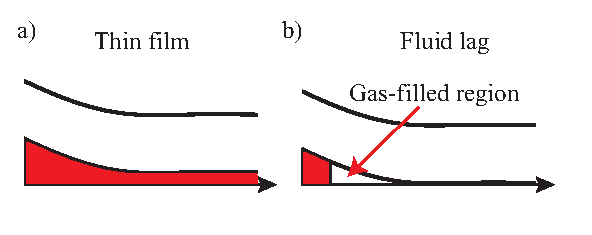
\includegraphics[scale=1.3]{Sketch.eps}
    \caption{Two different  regularization condition  at the  front of
      the current: a) thin prewetting film with thickness $h_f$ b) gas
      -filled region.}
    \label{C7-Sketch}
  \end{center}
\end{figure}
In particular, they show that
\begin{eqnarray}
  h_0&\propto& h_f^{-1/7}\nu^{-2/7}L^{10/7}~(\text{Thin film})\\
  h_0&\propto& \sigma^{1/9}\nu^{-2/9}L^{14/9}~(\text{Fluid lag})
\end{eqnarray}
where $L$  is the half  length of the  flow, $-\sigma$ is  the contant
negative  pressure  in  the  fluid   lag  and  we  have  rescaled  the
characteristic    thickness    and     time    by    $\nu^{1/4}$    in
\citet{Anonymous:QWXp_4JV}.    As   expected,    the   two   different
regularization condition leads  to only minor change  in the thickness
to   length   relationship   ($10/7\sim  1.4$,   $14/9\sim   1.5   $).
Nevertheless, a  complete description of  the dynamics of  the cooling
gas-filled region,  whose dynamics would depend  on temperature, might
also be required.

In the end, further works should  coupled the model derived in Chapter
\ref{C3-JFM} and  \ref{Heating} to a  more careful description  of the
different processes  involved at  the scale of  the current  tip. Such
approach should surely  give interesting insights and  a more complete
view of the dynamics of shallow magmatic intrusion.

\subsection{Further refinements for the model}

\subsubsection*{Viscous heating instabilities}

Viscous heating  is another mechanism  not taken into account  in this
study  that would  participate  to the  dynamics  of shallow  magmatic
intrusions. Indeed, especially for large  values of $Pe$ where we have
shown  that the  temperature  gradient within  the  flow are  stronger
(Section  \ref{C4-sec:infl-therm-bound-el}),  the  effect  of  viscous
heating could  be important.  \citet{Costa:2005bq} have  already shown
that viscous heating plays an important role in the dynamics of fluids
with strongly temperature-dependent viscosity. In particular, for lava
tube, they show that the heat generated by viscous friction produces a
local  temperature increase  near  the tube  walls  with a  consequent
decrease  of   the  viscosity   which  may  dramatically   change  the
temperature             and              velocity             profiles
\citep{Costa:2002cj,Costa:2003wk,Costa:2005bq}.      The     important
gradients near  the tip  region or within  the thermal  boundary layer
could  present  favorable  conditions  for  the  development  of  such
instabilities.

\subsubsection*{Stretching in the upper layer}

If the thickness of the intrusion  $h_0$ becomes large compared to the
intrusion depth $d_c$, the  analysis described in Chapter \ref{C3-JFM}
and  \ref{Heating}  is  not  valid  anymore. It  could  be  the  case,
especially for felsic intrusions characterized by large injection rate
intruding a layer such that $d_c\lessapprox 500$ m. In such situation,
the stretching  of the  upper layer  can no  longer be  neglected when
calculating the elastic stresses and  fluid pressure.  In that case, a
complete description  of the flow  in an axysimmetrical  and Cartesian
geometry for an isoviscous flow,  along with scaling laws for $h_0(t)$
and $R(t)$,  has already  been described by  \citet{Lister:2013ia} and
\citet{Anonymous:QWXp_4JV} respectively.  While the time dependence of
the scaling law are somewhat similar from those derived in the bending
dominated regime, the shape of the  flow is not bell-shaped anymore in
the early time solution and show a somewhat conical shape instead. For
instance, this  model could potentially  explain the conical  shape of
some     felsic      laccoliths     observed     in      Island     by
\citet{Anonymous:jHnLP36x}.
\begin{figure}[h!]
  \begin{center}
    \graphicspath{ {/Users/thorey/Documents/These/Manuscript/Figure/Chapter7/} }
    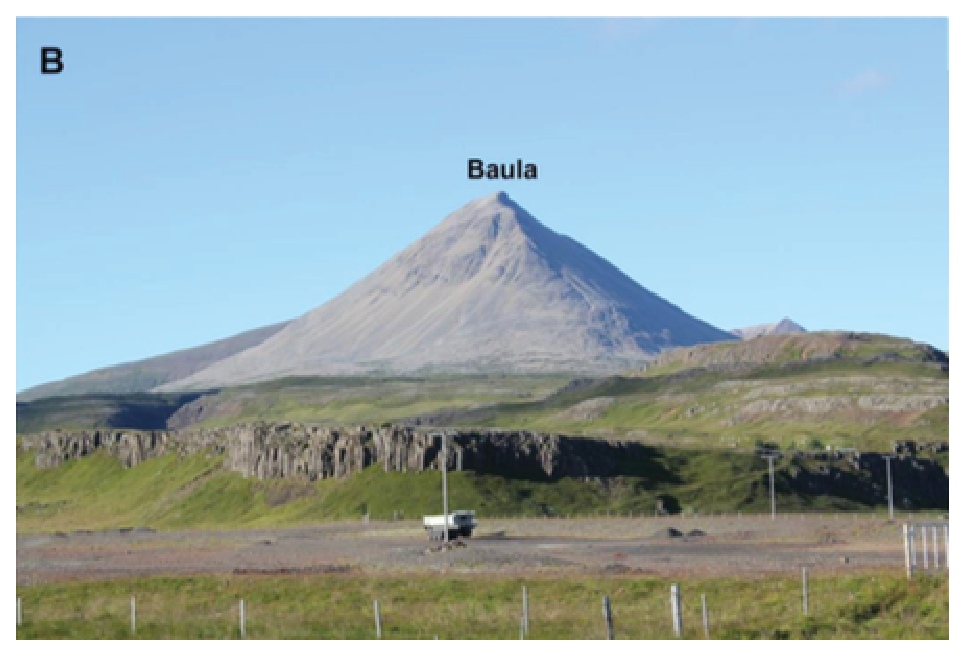
\includegraphics[scale=0.7]{Baula.eps}
    \caption{Felsic laccolith, named Baula,  in West Island.  Modified
      from \citet{Anonymous:jHnLP36x}.}
    \label{C7-Baula}
  \end{center}
\end{figure}

\subsubsection*{Contact aureole}

In chapter \ref{Heating},  we show that a  significant thermal aureole
should develop in the wall rocks above the central flow region.  Apart
from  plastic rock  deformation  that might  develop  in the  encasing
rocks,  studying  the  possible  thermal  erosion  could  also  be  an
interesting thing to look at. For instance, above the feeder dyke, the
temperature are  expected to be  maximum on  the roof and  might favor
subsequent dyke propagation. This could potentially explain the nested
structure of  several laccolith  complexes reported in  the literature
\citep{E:2015tl,Rocchi:2010dn}. Such  dyke formation would  also limit
the size of the terrestrial laccoliths.

\section{Lunar intrusive magmatism}
\label{sec:dynam-shall-magm}

While it provides for important  constraints on the Moon's thermal and
petrogenetic evolution,  the total  volume of  melt produced  into the
Moon interior is poorly known. In this thesis, we confirm the presence
of many shallow magmatic intrusion  in the lunar crust. In particular,
around  $10$ low-slope  lunar  domes and  about $200$  floor-fractured
craters have been detected at the  lunar surface, most of them located
close  or within  the lunar  maria. While  the total  volume of  these
magmatic intrusions should not exceed  $1\%$ of lunar maria volume, it
advocates the presence of numerous  shallow magmatic intrusions in the
lunar crust. This  suggests that deeper and  probably larger intrusion
might stands at the base of the lunar crust.



%%% Local Variables:
%%% mode: latex
%%% TeX-master: "../main"
%%% End:

